\chapter{Measuring control in hypergraphs}
\label{ch:MeasuringHypergraphControl}

The development of the relational perspective has allowed us to formulate the fundamentals of socially structured economies. We provided a network-institutional analysis of socio-economic interaction and, from this basis, developed a theory of entrepreneurship and the entrepreneurial function. The interaction between entrepreneurs and their unique positional attributes was noted and developed with respect to simple network configurations that express a Platonian economy. This chapter builds from the network analysis conducted in Parts~\ref{part:generalTheoryEntrepreneurship} and~\ref{part:entrepreneurshipPlatonianEconomy} by creating a measurement of control within a more complex socio-economic space; one that is representative of a Platform economy.

We defined entrepreneurship in a general way as an action or set of actions that modify, in a major way, elements of the socio-economic space; including the governance system and interaction infrastructure. This process can lead to the development of new socio-economic roles and the formation of exploitive positions in the underlying network of social and economic relations. Although this chapter does not try to address the institutional factors of entrepreneurship, it does provide a set of tools to investigate agents that attain powerful and potentially exploitative positions within complex spaces. These tools are exercised in the the subsequent chapter wherein we investigate individuals and firms that achieved exceptional power and, with it, provoked huge institutional change. The aim of this chapter should therefore be clear: to develop a set of tools that measure the power of agents within a complex network environment. This complex environment is represented by a \emph{hypergraph}; a structure that contains both individuals nodes and affiliation structures. We achieve this aim through the construction of the $\sigma$-score; a measurement that generalises both the standard degree measure and the $\beta$-measure. The $\sigma$-score is further generalised for use in weighted hypergraph environments. The ultimate goal of this measure within this monograph is to be used to investigate directorate networks, which is done in Chapter~\ref{ch:ControlInNYC}.

We add further complexity to the interaction infrastructure by integrating the notion of \emph{aspectual hypergraphs}: hypergraphs that contain nodes of many different types. In our case we can see populations of nodes of different socio-economic roles. This is again brought to life through the analysis of directorate networks. From the notion of aspects we arrive at a theory of \emph{elites}: individual nodes that exist in all aspects of a socio-economic space. This terminology is, of course, inspired by the elite Florentine families discussed in previous chapters. Not only did these families contain prestigious financiers, but individual family members were also industrialists, influential politicians, and overall Renaissance Men. This is a quality encapsulated by Cosimo di'Bicci de'Medici. Again, the eliteness of individual agents carries a lot of importance when investigating directors in the next chapter of the monograph.

\paragraph{Chapter outline.}

Section~\ref{Theory:Influence} introduces hypergraphs, networks, and other preliminary concepts. The section then provides some bespoke ways in which to measure the influence of individual nodes and affiliations in hypergraphs and network projections. Section~\ref{Theory:Elites} introduces aspectual hypergraphs, analyses and provides measures for the relatedness between aspects, and finally defines elites and elite structures.

\section{Centrality and influence in hypergraphs} 
\label{Theory:Influence}

\citet{Freeman1977} and~\citet{Bonacich1972} were first to develop measures of network centrality that are still commonly used network science\footnote{For more information on commonly used node centrality measures consider \citet[Chapter~2]{Jackson2008}.}. The degree and eigenvector centrality measures provide the foundation for other centrality measures that have been subsequently developed. The most common, the degree centrality, is determined by the number of links a given node has, and the eigenvector centrality measure is determined by the number of links that a node has and the number of links that each of its neighbours have. PageRank centrality~\citet{BrinPage1998} develops a measure that is built from eigenvector centrality; it specifically discounts the importance of a nodes link by the number of other connections the node has. These common measures of centrality have been applied to many different social and economic contexts, and have had application to directorate networks~\citep{Khanna2015, ElKhatib2015}.

Of specific interest to this chapter is the work of \citet{BrinkGilles1996, BrinkGilles2000}. The authors develop a measure of node dominance, known as the $\beta$-measure, which leads to an axiomatic generalisation of degree centrality in a directed network. The measure has had specific application to tournaments and games. \citet{BormBrink2002} develop an iterated $\beta$-measure which, much like the eigenvector and PageRank centralities, develops a score based on the dominance of the nodes that it dominates. With respect to hypergraphs, \citet{Corominas-MurtraThurner2014} develop a mechanism in which to identify the weak core and the structure of important nodes within a multidimensional network. Nodes that exist within a $k$-core and within multiple dimensions of the network are termed as elites: these elites will exist within a so-called \emph{rich club} \citep{Colizza2006}.

We construct a number of measures that compute the control of individual nodes and affiliations. Although the measures developed are general they are created to have particular application to interlocking and overlapping directorates. To do this we first introduce some preliminary concepts, such as hypergraphs and hypergraph projections. From this we can investigate degree-based centrality measures, and extend these to incorporate the influence of individuals and affiliations. This provides the structure for this section.

\subsection{Preliminaries}

\subsubsection*{Hypergraphs}

Let $N = \{ 1, \ldots ,n \}$ be a finite set of \emph{nodes}. An \emph{affiliation} is any subset $H \subset N$ of nodes. Technically, an affiliation is defined as a hyperlink on node set $N$.

A hypergraph is a node set endowed with a set of affiliations. Formally, a \emph{hypergraph} is now a pair $(N, \Gamma )$, where
\begin{equation}
\Gamma \subset \{ H \mid H \subset N \mbox{ and } H \neq \varnothing \} \equiv 2^N \setminus \{\varnothing\} ,
\end{equation}
and $| \Gamma | = h$ where $| \Gamma |$ denotes the number of elements in the finite set $\Gamma$.

A hypergraph thus represents an affiliation situation in which individuals, represented as nodes, are organised into affiliations, represented by hyperlinks\footnote{An alternative way to investigate hypergraph environments is through the use of a bipartite network, a concept we initially defined in Definition~\ref{def:bipartiteNetworks} when formalising interaction infrastructures in the socio-economic space.}. Usually we will use the shorthand notation $\Gamma$ as the hypergraph or affiliation situation where the node set $N$ is unambiguous.

We can formally define an ``affiliation situation'' as the class of all hypergraphs, $\mathbb{H}$, as
\begin{equation}
\mathbb{H}^N = \{ \Gamma \mid \Gamma \subset 2^N \mbox{ is an affiliation situation on } N \} .
\end{equation}

\paragraph{Neighbourhoods.}

Let $\Gamma \subset 2^N$ be some hypergraph. Then the \emph{affiliation set} of $i \in N$ is defined by
\begin{equation}
\Gamma_i = \{ H \in \Gamma \mid i \in H \}
\end{equation}
Thus, the affiliation set of a node is simply the collection of affiliations that it is a member of. This naturally leads to the identification of all nodes or individuals that a node encounters in its affiliations. The \emph{neighbourhood} of a node $i \in N$ is defined by
\begin{equation}
\overline{\Gamma}_i = \cup \Gamma_i \setminus \{ i \}
\end{equation}
The neighbourhood of a node is the set of nodes that are members of the affiliations that the node is involved with.

\paragraph{Overlapping affiliations.}

We allow that individual nodes can participate in multiple affiliations. The outcome is the overlap of multiple affiliations through a set of mutual nodes. It is clear that a set of affiliations, $\mathcal{H} \subseteq \Gamma$, are \emph{overlapping} if
\begin{equation}
\bigcap_{H \in \mathcal{H}} H \neq \varnothing .
\end{equation}
The \emph{environment} of $H \in \Gamma$, denoted by $\mathcal{E}_{H}$, is given as
\begin{equation}
\mathcal{E}_{H} = \{K \in \Gamma \, \mid \, K \cap H \neq \varnothing \mbox{ and } K \neq H \} .
\end{equation}
$\mathcal{E}_{H}$ is the largest set of overlapping affiliations containing $H$.

\paragraph{Weighted hypergraph.}

A hypergraph structure can be generalised by adding a weight to each affiliation; the result of which is a \emph{weighted hypergraph}, denoted by $\Gamma'$, in which the weight of some $H \in \Gamma$ is given by some real number which is denoted by $\nu_{H} \in \mathbb{R}$. A weighted hypergraph is therefore defined by the triple $\Gamma' = (N, \Gamma, \mathbf{v})$ where $N$ and $\Gamma$ are the set of nodes and affiliations respectively, as defined above, and $\mathbf{v} = (\nu_{1}, \ldots , \nu_{h})$ is a vector of weights that are attached to each affiliation.

Much like above, we can define a `weighted affiliation situation' as:
\begin{equation*}
\mathbb{L}^N = \{ \Gamma' \mid \Gamma' \subset 2^N \times \mathbf{v} \mbox{ is a weighted affiliation situation on } N \} ,
\end{equation*}
The weight of an affiliation can refer to the intensity of the relationship between its members, such that a larger weight denotes a greater intensity. Within our context, however, the weight of the affiliation specifically denotes the ``economic value'' of the affiliation. More specifically, as discussed in the application below, the weight of a firm refers to the value of the firms' total assets.

\begin{figure}[t]
\begin{center}
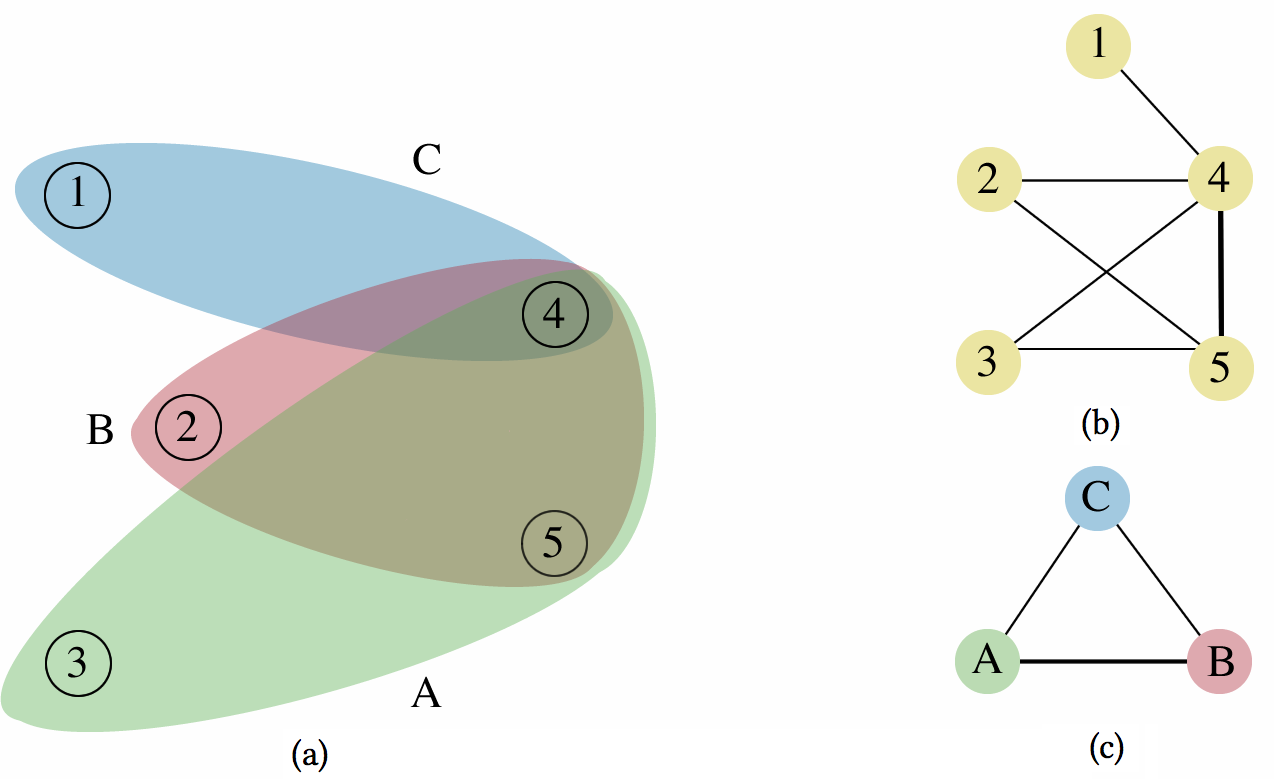
\includegraphics[scale=0.28]{Images/hypergraph.png}
\end{center}
\caption[Hypergraph and network projections]{Figure (a) is a hypergraph containing five nodes and three affiliations. Network (b) is the affiliation projection of hypergraph (a). Network (c) is the node projection of hypergraph (a).}
\label{hypergraph}
\end{figure}

\subsubsection*{Networks}

A hypergraph can be projected into two networks: the first is a \emph{node projection} and the second is an \emph{affiliation projection}. The projections are represented as networks and therefore we use the term `network' and `projection' interchangeably.

\paragraph{Node projection.}

A hypergraph can be projected on the node set $N$. A node projection of the hypergraph $\Gamma$ is denoted by $g_N$, which refers to the set of relationships $g_N = \{ij \, \mid \, j \in \overline{\Gamma}_{i} \mbox{ and } i \neq j \}$, where $ij$ is an \emph{undirected link} between nodes $i$ and $j$, such that $ij = ji$, therefore if $ij \in g_{N}$ then $ji \in g_{N}$. The node network from the hypergraph in Figure~\ref{hypergraph} (a) can be seen in Figure~\ref{hypergraph} (b).

\paragraph{Affiliation projection.}

Furthermore, a hypergraph can be projected into an affiliation projection on the set of affiliations, $\Gamma$. An affiliation network of the hypergraph $\Gamma$ is denoted by $G_{\Gamma}$, which refers to a set of reciprocated \emph{arcs} $G_{\Gamma} = \{ HK \, \mid \, K \in \mathcal{E}_{H} \mbox{ and } H \in \Gamma \}$. The affiliation network from the hypergraph in Figure~\ref{hypergraph} (a) can be seen in Figure~\ref{hypergraph} (c).

Links between the set of nodes in the node projection of a hypergraph can have a weight determined by the number of mutual affiliations between the nodes. Moreover, the arcs in the affiliation projection can have a weight determined by the number of mutual nodes between the affiliations. Formally, with respect to the node projection, the weight on an a link between a pair of nodes $i,j \in N$ is given by
\begin{equation} \label{eq:nodeweight}
\omega_{ij}(\Gamma) = | \overline{\Gamma}_{i} \cap \overline{\Gamma}_{j} | .
\end{equation}
Also, with respect to the affiliation projection, the weight on an arc from affiliation $H \in \Gamma$ to another affiliation $K \in \Gamma$ is given by
\begin{equation} \label{eq:affweight}
\omega_{HK}(\Gamma) = | H \cap K | .
\end{equation}
If $\omega_{ij}(g_{N}) = 0$ then there does not exist a weighted undirected link between nodes $i$ and $j$. Likewise, if $\omega_{HK}(G_{\Gamma}) = 0$ then there exists no weighted arc from $H$ to $K$.

\subsection{Degree-based centrality measures in affiliation situations} 
\label{degreecentralities}

We provide a centrality measure for nodes and affiliations within the context of a hypergraph to be used in the analysis of empirical situations. The measure is directly related to the dependence of the affiliation on the individual node and the value of the affiliation(s) that the node is a member of. We use this to measure the influence of individual nodes and affiliations within a hypergraph.

Given the ultimate application of these measures to directorate networks we can interpret `influence' as the ability for agents to control resources. Indeed, this has particular importance with regard to directorate hypergraphs whereby the influence of a director is given by the voting rights of the director and the size of the firm(s) that they are members of. Indeed, having proportionally more voting rights to the decisions of a firm and/or being a board member of a highly valued firm will increase a directors influence on the resources that the firm owns. From this we can derive the external influence of an affiliation or firm, which refers to the total amount of resources that it can potentially control beyond itself. We define the influence of an individual or affiliation---given by the $\sigma$-score---in its most general form as a centrality measure on a hypergraph.
\begin{definition}
Let $N = \{ 1, \ldots ,n \}$ be a given set of nodes. A \textbf{centrality measure} on $N$ is a function $\varphi \colon N \times \mathbb{H}^N \to \mathbb{R}^N$.
\end{definition}
A centrality measure on $N$ is a function that for every affiliation situation represented by a hypergraph $\Gamma \subset 2^N$ assigns to every individual node $i \in N$ a real number $\varphi_i ( \Gamma )$ representing the importance of $i$ in $\Gamma$. Ideally the measure should correctly represent the importance of an individual in the corporate situation represented by $\Gamma$.

There exists no specific measure of centrality for hypergraphs; most measures are either derived from the degree of the node or derived from the paths and walks that a node lies on. We specifically focus on degree-based measures, elaborating on the standard degree measure, the generalised $\beta$-measure, and influence.

\subsubsection*{Standard degree measure}

The \emph{standard degree measure} is the centrality measure $\delta \colon N \times \mathbb{H}^N \to \mathbb{R}^N$, which for every node $i \in N$ is defined by
\begin{equation}
\delta_i (\Gamma ) = \left| \overline{\Gamma}_i \right| .
\end{equation}
For general hypergraphs the sum of the standard degree across all nodes is computed as
\begin{equation}
\sum_{i \in N} \delta_i (\Gamma ) = \sum_{H \in \Gamma} | H | \, ( \, | H | - 1) - \sum_{H,H' \in \Gamma} | H \cap H' | \cdot \frac{| H \cap H' | - 1}{2} .
\end{equation}
For hypergraphs where $| H | = 2$ for all $H \in \Gamma$, this simplifies to $\sum_{i \in N} \delta_i (\Gamma ) = \sum_{H \in \Gamma} | H | \, ( \, | H | - 1) = 2 \, | \Gamma |$. These are networks.

If $\Gamma$ is projected as a node network, $g_N$, the standard degree measure simplifies to the standard degree concept defined and used in network analysis given by
\begin{equation}
\delta_i (\Gamma ) = d_i (g_N ) = | \, \{ j \in N \mid \, j  \in \Gamma_{i} \mbox{ where } j \neq i \}  \, |.
\end{equation}
Likewise, for node projected hypergraphs where $| H | = 2$ for all $H \in \Gamma$ in the initial hypergraph, $\sum_{i \in N} d_i (g_{N}) = 2 \, | \Gamma |$.

Finally, we denote the degree of an affiliation, $H \in \Gamma$, in the affiliation projection of $\Gamma$ as $\delta_{H}(G_{\Gamma}) = | \mathcal{E}_{H} |$, or simply as $\delta_{H}$.

\subsection{A hypergraph $\beta$-measure}

The \emph{hypergraph} $\beta$-\emph{measure} is the centrality measure $\beta \colon N \times \mathbb{H}^N \to \mathbb{R}^N$ given by
\begin{equation}
\beta_i (\Gamma ) = \sum_{j \in \overline{\Gamma}_i} \frac{1}{\left| \, \overline{\Gamma}_j \right|}
\end{equation}
In the case that $\Gamma$ is a network on $N$ this simplifies to
\begin{equation}
\beta_i (g_{N}) = \sum_{j \in \overline{\Gamma}_i} \frac{1}{d_j (\Gamma )} \equiv \beta_i (\Gamma ) .
\end{equation}
which is indeed equivalent to the original formulation of the $\beta$-measure for networks by \citet{BrinkGilles2000}. The $\beta$-measure is a measure of dominance whereby some node, $i$, dominates another, $j$, if $ij \in g_{N}$ or $\Gamma_{i} \cap \Gamma_{j} \neq \varnothing$. The total dominance distributed across the node set of the hypergraph is given by the total number of nodes that participate in at least one affiliation. We note this formally as
\begin{equation}
\sum_{i \in N} \beta_{i}(\Gamma) = | ~ \{ i \in N ~ | ~ \Gamma_{i} \neq \varnothing \} ~ | .
\end{equation}
The standard $\beta$-measure can be supported as a Shapley value of a corresponding TU-game describing the power relations in an affiliation situation.\footnote{A TU-game or ``cooperative game with transferable utilities'' on the node set $N$ is a function $v \colon 2^N \to \mathbb{R}$ such that $v( \varnothing )=0$. It describes the values that can be generated by groups of nodes in the affiliation situation under consideration. The \emph{Shapley value} of a TU-game $v$ is defined as $\phi_i (v) = \sum_{S \colon i \in S} \frac{\Delta_v (S)}{|S|}$, where $\Delta_v (S) = \sum{T \subset S} (-1)^{|S|-|T|} v(T)$ is the \emph{Harsanyi dividend} of the coalition $S$ in the game $v$.}
\begin{theorem}
Let $\Gamma$ be some affiliation situation on node set $N$. We define $V_{\Gamma} \colon 2^N \to \mathbb{R}$ as the TU-game given by
\begin{equation}
v_{\Gamma} (S) = \left| \, \cup_{j \in S} \overline{\Gamma}_j \, \right| .
\end{equation}
Then the Shapley value of $V_{\Gamma}$ coincides with the $\beta$-measure for $\Gamma \colon$
\begin{equation}
\phi_i \left( V_{\Gamma} \right) = \beta_i (\Gamma ) .
\end{equation}
\end{theorem}
\begin{proof}
This proof follows the outline of the proof of a corresponding result for the $\beta$-measure for networks given in \citet{Gilles2010}.
\\
Let $\Gamma \subset 2^N$ be some affiliation situation on $N$. For every node $i \in N$ we define a TU-game $w_i \colon 2^N \to \mathbb{R}$ by
\begin{equation}
w_i (S) = \left\{
\begin{array}{ll}
1 & \mbox{if } S \cap \overline{\Gamma}_i \neq \varnothing \\
0 & \mbox{otherwise}
\end{array} \right. .
\end{equation}
Then it is clear that for every $S \subset N$
\begin{equation}
V_{\Gamma} (S) = \sum_{i \in N} w_i (S) \quad \mbox{or} \quad V_{\Gamma} = \sum_{i \in N} w_i
\end{equation}
and, therefore, by additivity of the Shapley value it holds that for every $j \in N \colon$
\begin{equation}
\phi_j \left( V_{\Gamma} \right) = \sum_{i \in N} \phi_j \left( w_i \right) .
\end{equation}
We can determine that the Harsanyi dividends for $w_i$ are given by $\Delta_{w_i} (S) = (-1)^{|S|+1}$. Therefore,
\begin{equation}
\phi_j (w_i) = \sum_{S \subset N \colon j \in S} \frac{\Delta_{w_i} (S)}{|S|} = \sum_{S \subset \overline{\Gamma}_i \colon j \in S} \frac{(-1)^{|S|+1}}{|S|} .
\end{equation}
Hence, for every $j \in N \colon$
\begin{align*}
\phi_j \left( V_{\Gamma} \right) & = \sum_{i \in N} \phi_j (w_i) = \sum_{i \in N} \, \sum_{S \subset \overline{\Gamma}_i \colon j \in S} \frac{(-1)^{|S|+1}}{|S|} \\[1ex]
& = \sum_{i \in \overline{\Gamma}_j} \, \sum_{S \subset \overline{\Gamma}_i \setminus \{ i \} } \frac{(-1)^{|S|}}{|S|+1} \\[1ex]
& = \sum_{i \in \overline{\Gamma}_j} \, \sum^{D_i-1}_{t=0} \binom{D_i-1}{t} \, \frac{(-1)^t}{t+1}
\end{align*}
where we use the shorthand $D_i = \left| \overline{\Gamma}_i \right|$. Now,
\begin{align*}
\sum^{D_i-1}_{t=0} \binom{D_i-1}{t} \, \frac{(-1)^t}{t+1} & = \frac{-1}{D_i} \, \left[ \, \sum^{D_i}_{t=1} \binom{D_i}{t} \cdot (-1)^t \, \right] = \\[1ex]
& = \frac{-1}{D_i} \, \left[ \, \sum^{D_i}_{t=0} \binom{D_i}{t} \cdot (-1)^t -1 \, \right] = \\[1ex]
& = \frac{-1}{D_i} \, \left[ \, (1-1)^{D_i} -1 \, \right] = \frac{1}{D_i} .
\end{align*}
Therefore,
\[
\phi_j \left( V_{\Gamma} \right) = \sum_{i \in \overline{\Gamma}_j} \frac{1}{D_i} = \sum_{i \in \overline{\Gamma}_j} \frac{1}{\left| \overline{\Gamma}_i \right|} = \beta_j (\Gamma )
\]
This shows the assertion.
\end{proof}

\paragraph{Generalised $\beta$-measure.}

The $\beta$-measure can be generalised such that there can exist weights on the relations between the nodes. This is for specific application to weighted directed or undirected networks, however we can derive the $\beta$-scores of nodes given that there can exist weighted relations between nodes in the node projection of the hypergraph.

Let $\Gamma$ be a hypergraph on node set $N$, where $i,j \in N$, the \emph{generalised $\beta$-measure}, denoted by $\beta^{\star}_{i}(\Gamma)$ for some node $i$, is given by
\begin{equation}
\beta^{\star}_{i}(\Gamma) = \sum_{j \in \overline{\Gamma}_{i}} \frac{\omega_{ij}(g_{N})}{W_{j}(\Gamma)} ,
\end{equation}
where $\omega_{ij}(g_{N}) = | \Gamma_{i} \cap \Gamma_{j} |$, as in Equation~\ref{eq:nodeweight}, and $W_{i}(\Gamma) = \sum_{i \in \overline{\Gamma}_{j}} \omega_{ij}(\Gamma)$. The generalised $\beta$-measure distributes the dominance weight of a node proportional to the weights of the relations on which node $j$ is dominated. These weights emerge, as noted above, in the node projection of the hypergraph. A non-weighted network is equivalent to the weighted network with
\[
\omega_{ij}(g_{N} ) = \left\{
\begin{array}{ll}
1 & \mbox{if } \Gamma_{i} \cap \Gamma_{j}  \\
0 & \mbox{otherwise .}
\end{array} \right.
\]
But then $W_{j}(\Gamma) = d_{j}(\Gamma)$ for all $j \in N$ and $\omega_{ij}(\Gamma) = \omega_{ij}(g) \in \{0,1\}$, so $\beta^{\star}_{i}(\Gamma) = \beta_{i}(\Gamma)$. Thus, the generalised $\beta$-measure is indeed a generalisation of the $\beta$-measure.

With respect to the set of affiliations, we can measure their $\beta$-score in much the same way as with the generalised $\beta$-measure for the node set. Let $\Gamma$ be a hypergraph where $H, K \in \Gamma$ are affiliations and let
\begin{equation}
W_{K}(\Gamma) = \sum_{H \in \mathcal{E}_{K}} \omega_{HK}(G_{\Gamma}) ,
\end{equation}
where $\omega_{HK}(G_{\Gamma})$ is given by Equation~\ref{eq:affweight}. The generalised $\beta$-measure for affiliations is now given by
\begin{equation}
\beta^{\star}_{H}(\Gamma) = \sum_{K \in \mathcal{E}_{H}} \frac{\omega_{HK}(G_{\Gamma})}{W_{K}(\Gamma)} .
\end{equation}
Much like above, this leads to the property that $\sum_{H \in \Gamma} \beta^{\star}_{H} (\Gamma) = | ~ \{ H \in \Gamma ~ | ~ H \neq \varnothing \} ~ |$. We provide an axiomatisation of the generalised $\beta$-measure in Appendix~\ref{BetaAxiomatisation} below.

\subsection{A standard $\sigma$-score}

An alternative centrality measure is the \emph{$\sigma$-score} defined as the centrality measure $\sigma \colon N \times \mathbb{H}^N \to \mathbb{R}^N$ with for every node $i \in N \colon$
\begin{equation}
\sigma_i (\Gamma ) = \sum_{H \in \Gamma_i} \frac{1}{|H|}
\end{equation}
\begin{proposition} \label{prop:SG-degree}
Let $\Gamma$ be a hypergraph. If $| H | = 2$ for all $H \in \Gamma$, the $\sigma$-score becomes
\begin{equation}
\sigma_i (\Gamma ) = \tfrac{1}{2} \delta_i ( \Gamma ) ,
\end{equation}
meaning that $\sigma_{i}(G_{\Gamma}) = \tfrac{1}{2} d_{i} (G_{\Gamma})$ in the affiliation projection.
\end{proposition}
Due to Proposition~\ref{prop:SG-degree} the $\sigma$-score is to be viewed as a degree-based measure. In fact, in comparison with the standard degree measure, it is an alternative generalisation of the degree concept used in network analysis to the realm of hypergraphs or affiliation situations. Further still, we will show that the \emph{weighted $\sigma$-score} is a further generalisation of the generalised $\beta$-measure.

The normalisation of the $\sigma$-score on the node set $N$ of general hypergraphs is different from the normalisation of the degree measure and the $\beta$-measure. This normalisation is given by
\begin{equation} \label{eq:sigmanorm}
\sigma_{N} = \sum_{i \in N} \sigma_i (\Gamma ) = | \Gamma | .
\end{equation}
Equation~\ref{eq:sigmanorm} clearly indicates that the $\sigma$-score is a normalised degree measure that normalises to the number of affiliations in hypergraph $\Gamma$.

Regardless of both measures being degree-based Example~\ref{comparedegree} shows that different centrality measures can provide substantially different outcomes of relative node centrality. Specifically we note that the relative centrality of nodes changes with the measure that is given, with node $1$ becoming relatively more important surpassing nodes $2$ and $3$ when considering the $\sigma$-score.

\begin{example} \label{comparedegree}
Consider the hypergraph, $\Gamma $, on node set $N = \{ 1, 2, 3, 4, 5\}$ shown in Figure~\ref{hypergraph} (a). The standard degree measure on all nodes is given by the vector, $\delta(\Gamma ) = ( 1, 2, 2, 4, 3)$, the generalised $\beta$-measure on all nodes is given by the vector, $\beta^{\star}(\Gamma) = ( \frac{1}{5}, \frac{9}{20}, \frac{9}{20}, \frac{5}{2}, \frac{7}{5} )$, and the $\sigma$-score on all nodes is given by the vector, $\sigma(\Gamma ) = ( \frac{1}{2} , \frac{1}{3}, \frac{1}{3}, \frac{7}{6}, \frac{2}{3} )$.
% Add the standard beta-score
\end{example}

The substantial differences mean that both measures concern different traits of node connectivity that influence the importance of a node. Specifically, the $\sigma$-score is fundamentally tied to the quantity and context of affiliations that a node is embedded, and is thus more attuned to the affiliations of the hypergraph. On the other hand the standard degree and $\beta$-measures is only concerned with the resulting network structure from the existence of affiliations and each nodes' membership to these affiliations \footnote{We highlight a restriction of the $\sigma$-score by noting that, unlike the standard degree measure, it cannot be used with respect to general projections of a hypergraph to a node network. Indeed, whereas the standard degree measure has direct application to a node network, this is only true with the $\sigma$-score where $| H | = 2$ for all $H \in \Gamma$.}.

\paragraph{Weighted $\sigma$-score.}

The $\sigma$-score can be generalised for use in weighted hypergraphs defined by the triple $\Gamma' = (N, \Gamma, \mathbf{v})$. The generalised $\sigma$-score is defined as the centrality measure $\sigma' : N \times \mathbb{L}^{N} \rightarrow \mathbb{R}^{N}$, with for every node $i \in N$:
\begin{equation}
\sigma'_{i}(\Gamma' ) = \sum_{H \in \Gamma_{i}' } \frac{\nu_{H}}{| H |} .
\end{equation}
The normalisation of the weighted $\sigma$-score subsequently becomes
\begin{equation} \label{sigmanorm}
\sum_{i \in N} \sigma'_{i}(\Gamma' ) = \sum_{H \in \Gamma' } \nu_{H} = V(\Gamma').
\end{equation}
\begin{example} \label{weightedSG}
Let the hypergraph on node set $N = \{ 1, 2, 3, 4, 5\}$ shown in Figure~\ref{hypergraph} (a) be a weighted hypergraph $\Gamma'$ where $\nu_{A} = 21$, $\nu_{B} = 15$, and $\nu_{C} = 8$, such that $V(\Gamma') = \sum_{H \in \Gamma'} \nu_{H} = 44$. The normalised weighted $\sigma$-score for all nodes is given by the vector, $\sigma'(\Gamma' ) = ( \frac{1}{11}, \frac{5}{44}, \frac{7}{44}, \frac{4}{11}, \frac{3}{11} )$.
\end{example}
Example~\ref{weightedSG} shows that the weight of an affiliation can have an impact on the centrality of a node. Specifically node $1$ now becomes relatively less important than both nodes $2$ and $3$, and there is a differential that emerges between nodes $2$ and $3$.

Where the value of an affiliation may matter, as in directorate networks, the initial $\sigma$-score bias the centrality of nodes. Specifically, nodes that are members of an affiliation with a small population (such as in the case with node $1$) may have a large centrality regardless of the value of the affiliation that they are members of. Further biases can emerge in the other direction whereby nodes that are members of affiliations with a large population could have a downward bias on their centrality.

\medskip \noindent To this point the $\sigma$-score has been applied to nodes only. This is extended to affiliations such that the $\sigma$-score of an affiliation within a weighted hypergraph is given by
\begin{equation}
\sigma_{H}(\Gamma') = \left( \sum_{K \in \mathcal{E}_{H}} \nu_{K} \cdot \frac{| H \cap K |}{| K |} \right) + \nu_{H},
\end{equation}
which simplifies to
\begin{equation}
\sigma'_{H}(\Gamma' ) = \sum_{i \in H} \sigma'_{i}(\Gamma ' ).
\end{equation}

\begin{example} \label{ex:influence}
Consider the weighted hypergraph, $\Gamma '$, on node set $N = \{ 1, 2, 3, 4, 5\}$ from Example~\ref{weightedSG} where $\nu_{A}(\Gamma' ) = 21$, $\nu_{B}(\Gamma' ) = 15$, $\nu_{C}(\Gamma' ) = 8$, and $V (\Gamma' ) = 44$. The normalised $\sigma$-score of each affiliation is given by the vector, $\Sigma(\Gamma' ) = ( \frac{35}{44}, \frac{3}{4}, \frac{5}{11} )$.

Furthermore we also highlight the relationship between the $\sigma$-score of the affiliations and the $\sigma$-scores of the individual nodes. From Example~\ref{weightedSG} we find that $A = \{3,4,5\}$ and $\sigma_{3}(\Gamma') + \sigma_{4}(\Gamma') + \sigma_{5}(\Gamma') = \frac{7}{44} + \frac{4}{11} + \frac{3}{11} = \frac{35}{44} \equiv \Sigma_{A}(\Gamma')$; $B = \{2,4,5\}$ and $\sigma_{2}(\Gamma') + \sigma_{4}(\Gamma') + \sigma_{5}(\Gamma') = \frac{5}{44} + \frac{4}{11} + \frac{3}{11} = \frac{3}{4} \equiv \Sigma_{B}(\Gamma')$; and finally $C = \{1,4\}$ and $\sigma_{1}(\Gamma') + \sigma_{4}(\Gamma') = \frac{1}{11} + \frac{4}{11} = \frac{5}{11} \equiv \Sigma_{C}(\Gamma')$.
\end{example}

Note that there does not always exist a relative relationship between the $\sigma$-score of an affiliation and its value in the weighted hypergraph. Moreover, this phenomenon may also not exist for the so-called external influence of the affiliation\footnote{The external influence of an affiliation only takes into consideration the influence that the affiliation has beyond itself.}. The \emph{external influence} of some affiliation $H \in \Gamma$ is given by
\begin{equation}
\sigma^{\star}_{H}(\Gamma' ) = \sigma'_{H}(\Gamma' ) - \nu_{H}
\end{equation}
In the case of Example~\ref{ex:influence} affiliation $B$ has the highest external influence even though affiliation $A$ has the highest value.

\begin{property} \label{prop:norm}
Let $\Gamma$ be a hypergraph on node set $N$ and $G_{\Gamma}$ be the affiliation projection of $\Gamma$.
\begin{abet}
\item $\sum_{i \in N} \sigma_{i}(\Gamma) = | ~ \{ H \in \Gamma~|~H \neq \varnothing \} ~ | = | \Gamma |$.

By extension, $\sum_{i \in N} \sigma_{i}(\Gamma') = \sum_{H \in \Gamma'} \nu_{H}$.

\item $\sum_{H \in \Gamma} \sigma_{H}(\Gamma) = | \Gamma | + \sum_{H \in \Gamma} \left( \sum_{K \in \mathcal{E}_{H}} \frac{| H \cap K |}{|K|} \right)$.

By extension, $\sigma_{\Gamma}(\Gamma') = \sum_{H \in \Gamma} \sigma_{H}(\Gamma') = V(\Gamma') + \sum_{H \in \Gamma} \left( \sum_{K \in \mathcal{E}_{H}} \nu_{K} \cdot \frac{| H \cap K |}{|K|} \right) $.

% This simplifies to $\sigma_{\Gamma}(\Gamma) = 2 | \Gamma |$ and $\sigma_{\Gamma}(\Gamma') = 2 V(\Gamma')$ if $| \Gamma_{i} | > 1$ and $\nexists ~ \mathcal{H} \subseteq \Gamma'$ such that $\cup \mathcal{H} = \varnothing$ and $| H | > 1$ for all $H \in \mathcal{H}$.
\end{abet}
\end{property}

In non-weighted hypergraphs, $\Gamma$, $\nu_{H} = 1$ for all $H \in \Gamma$. The weighted $\sigma$-score is equivalent to the $\sigma$-score when standardising all affiliation weights to 1, suggesting that the weighted $\sigma$-score is a generalised version of the $\sigma$-score.

\subsubsection*{Equivalence between the $\sigma$-score and the $\beta$-measure}

When considering the affiliation projection of the non-weighted hypergraph there emerges an equivalence between the $\sigma$-score and the $\beta$-measure of affiliations. We note that the $\beta$-score of some $H \in \Gamma$ in the affiliation projection $G_{\Gamma}$ is given by
\begin{equation}
\beta^{\star}_{H}(G_{\Gamma}) = \sum_{K \in \mathcal{E}_{H}} \frac{\omega_{HK}(G_{\Gamma})}{W_{K}(G_{\Gamma})} ,
\end{equation}
where $W_{K}(G_{\Gamma}) = \sum_{H \in \mathcal{E}_{K}} \omega_{HK} (G_{\Gamma})$.

The $\sigma$-score of an affiliation in the affiliation projection of a non-weighted hypergraph is given by
\begin{equation}
\sigma_{H}(G_{\Gamma}) = \left( \sum_{K \in \mathcal{E}_{H}} \omega_{HK}(G_{\Gamma}) \right) + 1
\end{equation}
Therefore, $\beta^{\star}_{H}(\Gamma) = \sigma_{H}(\Gamma) - 1$ if $W_{K}(G_{\Gamma}) = 1$ for all $K \in \mathcal{E}_{H}$. Example~\ref{ex:equiv} highlights this equivalence between the generalised $\beta$-measure and $\sigma$-score.

\begin{example} \label{ex:equiv}
Consider the hypergraph $\Gamma$ in Figure~\ref{hypergraph}(a) and the affiliation projection, $G_{\Gamma}$, in Figure~\ref{hypergraph}(c). The weights attached to the arcs were calculated in Example~\ref{comparedegree}; from these the generalised $\beta$-measure and $\sigma$-score for each affiliation can be calculated.

$W_{A}(G_{\Gamma}) = W_{B}(G_{\Gamma}) = W_{C}(G_{\Gamma}) = 1$ meaning that $\beta^{\star}_{A}(G_{\Gamma}) =\beta^{\star}_{B}(G_{\Gamma}) = \frac{7}{6}$ and $\beta^{\star}_{C}(G_{\Gamma}) = \frac{2}{3}$. Likewise, $\sigma_{A}(G_{\Gamma}) = \sigma_{B}(G_{\Gamma}) = \frac{13}{6}$ and $\sigma_{C}(G_{\Gamma}) = \frac{5}{3}$. Therefore, $\beta_{H}(G_{\Gamma}) = \sigma_{H}(G_{\Gamma}) - 1$ for all $H \in \Gamma$.
\end{example}

\section{Hypergraphs with aspects} \label{Theory:Elites}

We introduce the notion of \emph{aspectual hypergraphs}, i.e., hypergraphs with aspects. In general an \emph{aspect} refers to a set of nodes, or affiliations, categorised by a certain observable or well-defined characteristic. Specifically in our case we define an aspect as a certain division of labour that an affiliation specialises in; it is therefore comparable to an industry within which a set of firms operates in. The aspect(s) to which each individual node participates is derived from the set of affiliations that they are members of and the aspects that the affiliations are subsequently embedded in.

\subsection{Aspectual hypergraphs}

\paragraph{Aspectual hypergraphs.}

The set of \emph{aspects} in a hypergraph is given by
\begin{equation}
\mathcal{A} = \{ A ~ | ~ A \subseteq \Gamma \mbox{ and } A \cap A' = \varnothing \mbox{ for any } A' \subseteq \Gamma \} ,
\end{equation}
where $| \mathcal{A} | = a$. Subsequently, an \emph{aspectual hypergraph} is defined by the triple $\Gamma_{\mathcal{A}} = (\Gamma, N, \mathcal{A})$ and, for completeness, a \emph{weighted aspectual hypergraph} is defined by the quadruple $\Gamma'_{\mathcal{A}}= (\Gamma, N, \mathbf{v}, \mathcal{A})$.

We let $\mathcal{A}_{H} = \{ A \in \mathcal{A} \, \mid \, H \in A\}$ and $\mathcal{A}_{H} \neq \varnothing$ for all $H \in \Gamma$. We highlight the restriction such that $| \mathcal{A}_{H} | = 1$ for all $H \in \Gamma$, which provides disjointed partitions of affiliations into aspectual spaces\footnote{However the restriction could be weakened for future work.}.

Nodes also operate in at least one aspect as a consequence of being a member of more than one affiliation. The set of aspects that some $i \in N$ operates in is given similarly given by $\mathcal{A}_{i} = \{ A \in \mathcal{A}_{H} \, \mid \, i \in H \}$. The player set of a given aspect $A \in \mathcal{A}$ is given as $N(A) = \{ i \in N \, \mid \, i \in H \text{ and } \mathcal{A}_{H} = A \}$.

\subsubsection*{Aspectual distance}

Aspects can overlap with respect to their node set. The degree in which a pair of aspects overlap is determined by the number of nodes associated with both aspects.

\begin{definition}
The \textbf{distance} between a pair of aspects, $A$ and $A'$, is given by:
\begin{equation}
\mbox{dist}(A, A',\Gamma_{\mathcal{A}}) = 1 - \frac{| N(A) \cap N(A') |}{| N(A) |} ~ ,
\end{equation}
where $\mbox{dist}(A, A',\Gamma_{\mathcal{A}}) \in [0,1]$.
\end{definition}

If $N(A) \subseteq N(A')$, then $\mbox{dist}(A, A', \Gamma_{\mathcal{A}}) = 0$; therefore, the more overlapping a pair of aspects then the closer to $0$ the distance between the aspects will be. Note, $\mbox{dist}(A, A',\Gamma_{\mathcal{A}}) = \mbox{dist}(A, A',\Gamma_{\mathcal{A}}) \iff | N(A) | = | N(A') |$.

The overlap of aspects provides an indicator for how many bridge relations are contained between the aspects. As $\mbox{dist}(A, A',\Gamma_{\mathcal{A}}) \rightarrow 1$ then fewer bridge relations exist from aspect $A$ to aspect $A'$, meaning that if $\mbox{dist}(A, A',\Gamma_{\mathcal{A}}) = 1$ no bridges exist. If there are only a few nodes that intersect between aspects there must exist more power in those nodes to bridge relations between aspects. Conversely, if there are relatively many nodes in the intersection between the aspects, then there will be limited scope for brokerage between the aspects. Power to broker relations and information between aspects is centralised in the intersection between aspects.

\begin{example} \label{ex:dist}
Let the hypergraph on node set $N = \{1,2,3,4,5\}$ from Figure~\ref{hypergraph}(a) be an aspectual hypergraph $\Gamma_{\mathcal{A}}$. This hypergraph has an aspect set given by $\mathcal{A} = \{A_{1}, A_{2} \}$, where $A_{1} = \{A,B\}$ and $A_{2} = \{C\}$. Given this we calculate the asymmetrical distances to be $\mbox{dist}(A_{1}, A_{2}, \Gamma_{\mathcal{A}}) = \frac{1}{4}$ and $\mbox{dist}(A_{2}, A_{1}, \Gamma_{\mathcal{A}}) = \frac{1}{2}$. Node $4$ is the single broker between the two aspects.
\end{example}

The notion of aspectual bridging can be complemented with the `correlation' between aspects. Indeed, although power is centralised within the intersection of aspects---the bridging relations---they will be more valuable if the aspects are highly correlated with, and therefore complimenting of, each other.

\subsubsection*{Aspectual correlation}

Aspects can be alike such that fluctuations in their structure and value can be correlated with each other. The relationship to which aspects are correlated should therefore be considered in the context that they are analysed. Within this chapter we consider the correlation between aspects to be a function of how the value of an aspect and its affiliations change over time.

We let the value of some aspect, $A \in \mathcal{A}$, in some time period $t \in \{1,\ldots,T\}$ be given by
\begin{equation}
\mu(A_{t}) = \sum_{H \in A} \nu_{H}(\Gamma'_{\mathcal{A}} ) .
\end{equation}
The likeness between a pair of assets is computed in the conventional fashion through the calculation of the standard deviation and covariance of the values of each pair of aspects. Specifically, let the standard deviation of some aspect, $A$, be calculated as
\begin{equation}
\lambda(A) = \sqrt{\frac{\sum_{t=1}^{T} \left[ \mu(A_{t}) - \overline{\mu}(A) \right]^{2}}{T}} ~ ,
\end{equation}
where
\begin{equation}
\overline{\mu}(A) = \frac{\sum_{t=1}^{T} \mu(A_{t})}{T} ~ ,
\end{equation}
and $T > 0$ is the number of time periods. From this, the covariance of two aspects, $A,A' \in \mathcal{A}$, is calculated by:
\begin{equation}
Cov(A,A') = \frac{\sum_{t=1}^{T} \left[ \mu(A_{t}) - \overline{\mu}(A) \right] \cdot \left[ \mu(A'_{t}) - \overline{\mu}(A') \right]}{T} ~ .
\end{equation}
Thus, the \emph{aspectual correlation} between the two aspects is given as:
\begin{equation}
r(A,A',\Gamma'_{\mathcal{A}}) = \abs{ ~ \frac{Cov(A,A')}{\lambda(A) \cdot \lambda(A')} ~ } ~ ,
\end{equation}
such that $r(A,A',\Gamma'_{\mathcal{A}}) \in [0,1]$, since the absolute value of the correlation co-efficient is used. As $r(A,A',\Gamma'_{\mathcal{A}}) \rightarrow 1$ the relationship between aspects increases; a change in the value of one aspect is reflected in a change in the value of another. The absolute value of the correlation is used because, regardless of whether the relationship is positive or negative the relationship can be used to assess the connectivity of the aspects.

The relationship between a pair of aspects is therefore informed by the variance and covariance of the pairs values. This is a time-dependent measure, meaning that multiple time periods are required to provide a meaningful calculation. The calculation suggests that only the changes in the values over time are considered when measuring the relationship between aspects over time.

\medskip \noindent The importance of bridge relations between a pair of aspects is given by the product of the distance and correlation between them. Specifically, the importance of a bridge relation is formally given by:
\begin{equation}
\Lambda(A,A',\Gamma'_{\mathcal{A}}) = \mbox{dist}(A,A',\Gamma'_{\mathcal{A}}) \times r(A,A',\Gamma'_{\mathcal{A}}) ~ ,
\end{equation}
where $\Lambda(A,A',\Gamma'_{\mathcal{A}}) \in [0,1]$.

The power of the bridge relation is a scalar that corresponds to the benefit of operating within multiple aspects. The importance of bridge relations is therefore a positive function of the distance between the aspects that the relation is bridging and the correlation between those aspects.

If, for example, the distance between aspects increases with a given correlation, then the importance of bridge relations between the aspects will also increase. Conversely, if the correlation between aspects increases with a given distance, then the importance of the bridge relation increases.

\subsection{Elites and elite structures}

The importance of a node can be determined by both the structural attributes of the network--as shown by conventional measures of node centrality--and by the number of aspects that the node participates in. Section~\ref{degreecentralities} introduced and defined a number of measures of importance and centrality that were strictly increasing with the degree of the node or affiliation. Here we define a measure of importance that is not strictly increasing with the degree of the node. We consider the definition of an elite set of nodes as the collection of nodes that are embedded within all aspects of the network.

The set of elites, which can be derived from the aspectual hypergraph, is defined below.
\begin{definition}
Let $\Gamma_{\mathcal{A}}$ be an aspectual hypergraph on node set $N$ where affiliations are partitioned into aspects given by the class $\mathcal{A}$. The \textbf{elite set} is given by:
\begin{equation}
\mathcal{E} = \bigcap_{A \in \mathcal{A}} N(A) .
\end{equation}
Node $i \in N$ is an \textbf{elite} if and only if $i \in \mathcal{E} \subseteq N$, and therefore $\mathcal{A}_{i} = \mathcal{A}$.
\end{definition}
The notion of an elite is important because an elite will, by virtue of their direct links, have access to information regarding all aspects of the hypergraph. With respect to the application of directorate networks, a director who is a member of all aspects has direct access to information regarding all industries within the economy, and can therefore make more holistic and better informed decisions.

The measurement of elite is degree-based, but not strictly so. The relationship between the degree of a node in a hypergraph, i.e., the number of affiliations that it is a member of, and the likelihood that the node will be an elite is weakly monotonically increasing. Such a relationship can be seen in Appendix~\ref{A} whereby the probability of becoming an elite and the degree of the node is mapped. In Figure~\ref{RandSim1} the $x$-axes of the graphs show the proportion of affiliations that a node is a member of, and the $y$-axes show the probability of the node becoming an elite. We can see that it follows a typical binomial cumulative distribution function, which is characterised by the number of affiliations and the number of aspects for a given node degree.

\paragraph{Elite structure.}

The resulting set of elite nodes has a corresponding network structure. An \emph{elite structure} corresponds to the resulting network from the restricted set of nodes who are elite.

\begin{definition}
Let $\Gamma_{\mathcal{A}}$ be an aspectual hypergraph on node set $N$ and aspect class $\mathcal{A}$, where $g_{N}$ is the node projection of $\Gamma_{\mathcal{A}}$. The \textbf{elite structure} is given by the subnetwork $g_{\mathcal{E}}$, where
\begin{equation}
g_{\mathcal{E}} = \{ ij \in g_{N} ~ | ~ i,j \in \mathcal{E} \subseteq N \},
\end{equation}
\end{definition}

The elite structure is important with respect to directorate hypergraphs for two reasons. First, it highlights the proportion of directors, and their relations, that are embedded in multiple aspects of the economy. Second, if elites are embedded in multiple aspects together then they are more likely to have stronger relations and to share information between them; this structure is more likely to indicate a strong conduit of information dissemination. Arguably, centrality and brokerage in this network will be more reflective of power in the hypergraph.

\begin{subappendices}
\section{Axiomatisation of the generalised $\beta$-measure}
\label{BetaAxiomatisation}

The generalised $\beta$-measure can be characterised through the use of four axioms. We present these axioms on an arbitrary relational power measure $f : \mathbb{H}^{N} \rightarrow \mathbb{R}^{N}$, where any hypergraph structure, $\Gamma$, can be drawn from $\mathbb{H}^{N}$, that uniquely determine the generalised $\beta$-measure. These axioms are as follows.

\begin{axiom}[Weighted dominance normalisation] \label{ax:1}
For every $\Gamma \in \mathbb{H}^{N}$ it holds that
\[
\sum_{i \in N} f_{i}(\omega) = | ~ \{ j \in N ~ | ~ \lambda_{\omega}(j) > 0 \} ~ |
\]
\end{axiom}

\begin{axiom}[Weighted dummy node property] \label{ax:2}
For every $\Gamma \in \mathbb{H}^{N}$ and every $i \in N$ with $\Gamma_{i} = \varnothing$ it holds that $f_{i}(\omega) = 0$.
\end{axiom}

\begin{axiom}[Weight proportionality] \label{ax:3}
For every $\Gamma \in \mathbb{H}^{N}$ and every pair $i,j \in N$ for which there is a constant $c_{i,j} \in \mathbb{R}$ such that $\omega(i,h) = c_{i,j} \cdot \omega(j,h)$ for every $h \in N$ it holds that
\begin{equation}
f_{i}(\omega) = c_{i,j} \cdot f_{j}(\omega) ~ .
\end{equation}
\end{axiom}

To state the fourth axiom we introduce a partition of a hypergraph $\Gamma$ as a collection of hypergraphs $\mathcal{G} = \{\Gamma_{1}, \ldots, \Gamma_{m}\}$ such that $\sum_{\ell = 1}^{m} \omega_{ij}^{\ell} = \omega_{ij}$ for every $ij \in g_{N}$.


\begin{axiom}[Additivity over weighted independent partitions] \label{ax:4}
For every $\Gamma \in \mathbb{H}^{N}$ and independent partition $\mathcal{G}$ of $\Gamma$ it holds that
\begin{equation}
f(\omega) = \sum_{\omega_{k} \in \mathcal{G}} f(\omega_{k})
\end{equation}
\end{axiom}

The generalised $\beta$-measure satisfies these four axioms.

\section[Degree and probabilistic eliteness]{Node degree and the probability of being elite} \label{AppA}

The number of elites in a network is important when considering elite structures and the distance between aspects. Here, we assess the weakly positive monotonic relationship between the degree of a node and the probability that it is elite. This can also be translated in terms of influence: intuitively, as a nodes influence increases its probability of becoming an elite must also increases in a non-linear fashion.

The probability that a node is an elite loosely follows a binomial distribution. Specifically, let the probability that some node $i \in N$ is an elite be denoted very literally as $Pr(i \in \mathcal{E})$ then, given that $| \Gamma_{i} | = h_{i}(\Gamma) > 0$ and $i$ has a number of connections possible, the probability is given by:
\[
Pr(i \in \mathcal{E}) = \frac{\mbox{Number of correct combinations of $b_{i}(\Gamma)$ links}}{\mbox{Total number of combinations of $b_{i}(\Gamma)$ links}}.
\]
The total number of connection combinations on affiliation set $\Gamma$ is given by $\binom{h}{h_{i}(\Gamma)}$. The number of `correct' combinations refers to the number of ways in which node $i$ can become an elite. As discussed above, there is a conditions on $i$ to become an elite and there is a restriction placed on the network.

\begin{abet}
\item The condition is that $\mathcal{A}_{i} = \mathcal{A}$, therefore $h^{A}_{i}(\Gamma) \geqslant 1 \, \forall \, A \in \mathcal{A}$.

\item The restriction is that $h^{A}_{i}(\Gamma) \leqslant \alpha_{A} \, \forall \, \ell \in K$.
\end{abet}
Due to (a) and (b) the probability of a node becoming elite deviates from the typical binomial distribution. The probability follows a multivariate hyper-geometric distribution with the following probability mass function :
\begin{equation} \label{eq:PMF}
Pr(i \in \mathcal{E}) =  \left[ \prod_{A = 1}^{a} \dbinom{\alpha_{A}}{h^{A}_{i}(\Gamma)} \right] \cdot \dbinom{h}{h_{i}(\Gamma)}^{-1},
\end{equation}
where $| \mathcal{A} | = a$. With Equation~\ref{eq:PMF} we make the assumption that $h_{i}(\Gamma) \geqslant a$ and $\alpha_{A} \, \forall \, A \in \mathcal{A}$. Note that if $h_{i}(\Gamma) < a$ then $Pr(i \in \mathcal{E}) = 0$ due to the failure to satisfy condition (a).

All potential combinations for all $\alpha_{A}$ need to be assessed and plugged into the probability mass function above. For lack of a general formula to calculate the probability that a node is an elite given (a) and (b) an algorithm is developed to solve for the total number of correct combinations given $h_{i}(\Gamma) > 0$.

Before continuing with the algorithm we first define the set $C(h_{i}(\Gamma))$ as a set of affiliation combinations such that the number of affiliation is equal to $h_{i}(\Gamma)$. Formally,
\[
C(h_{i}(\Gamma)) = \left\{ \mathcal{H} \subseteq \Gamma \, \mid \, | \mathcal{H} | = h_{i}(\Gamma) \right\} .
\]
Note that there may be multiple distinct sets of affiliations that contain $h_{i}(\Gamma)$ distinct affiliations. We let the $v^{th}$ distinct set be denoted as $C^{v}(h_{i}(\Gamma))$. The algorithm is as follows:

\begin{abet}
\item[(1)] Construct the class $\mathcal{C}(h_{i}(\Gamma))$ as a set of sets containing all distinct sets of affiliations of size $h_{i}(\Gamma)$. Therefore:
\begin{align*}
\mathcal{C}(h_{i}(\Gamma)) & = \left\{ C(h_{i}(\Gamma)) \subseteq \Gamma \, \mid \, | C(h_{i}(\Gamma)) | = h_{i}(\Gamma) \right\}\\
                   & = \left\{C^{1}(h_{i}(\Gamma)), \ldots, C^{v}(h_{i}(\Gamma))\right\}
\end{align*}
in such a case $p = | \mathcal{C}(h_{i}(\Gamma)) | = \binom{m}{d_{i}}$.

\item[(2)] Construct sets $B \in \mathcal{C}(d_{i})$ such that all affiliations contained in each set $B$ are collectively members of all aspects. Therefore:
\[
B(h_{i}(\Gamma)) = \left\{ H \in \Gamma \, \mid \, B \cap A_{\ell} \neq \varnothing \, \forall \ell \in \mathcal{A} \mbox{ and } | B (h_{i}(\Gamma)) | = h_{i}(\Gamma) \right\} .
\]
Again, note that there may exist more than one set $B(h_{i}(\Gamma))$ that contains $h_{i}(\Gamma)$ distinct affiliations throughout all aspects. Similar to above, we let the $u^{th}$ distinct set be denoted as $H^{u}(h_{i}(\Gamma))$.

\item[(3)] Construct the class $\mathcal{H}(h_{i}(\Gamma)) \subseteq \mathcal{C}(h_{i}(\Gamma))$ as a set containing all $B(h_{i}(\Gamma))$. Therefore:
\[
\mathcal{B}(h_{i}(\Gamma)) = \left\{ B^{1}(h_{i}(\Gamma)), \ldots, B^{u}(h_{i}(\Gamma)) \right\}
\]
The set $\mathcal{B}(h_{i}(\Gamma))$ contains all combinations of affiliations that lead to node $i$ becoming an elite. If $h_{i}(\Gamma) < a$ then $\mathcal{B}(h_{i}(\Gamma)) = \varnothing$ and $u = 0$.

\item[(4)] Calculate:
\[
Pr(i \in \mathcal{E}) = \frac{ | \mathcal{B}(h_{i}(\Gamma)) |}{ | \mathcal{B}(h_{i}(\Gamma)) |} = \frac{u}{p} .
\]
\end{abet}

\begin{example} \label{ex:probelite}
Consider a hypergraph, $\Gamma$, with a set of nodes, $N$ where $|N| = 1$, a set of affiliations, $\Gamma$ where $| \Gamma | = 24$, and a set of aspects, $\mathcal{A}$ where $|\mathcal{A}| = 6$. The set of aspects are distributed evenly across all affiliations such that $\alpha_{A} = 4 \, \forall \, A \in \mathcal{A}$.
\end{example}

Note from Example~\ref{ex:probelite} above that the probability of node $i$ becoming an elite in weakly monotonic and loosely follows a typical binomial distribution.

\begin{proposition} \label{bounds}
Let $\Gamma$ be a hypergraph on node set $N$ and affiliation set $\Gamma$ where $i \in N$ and $|\Gamma| = h$. The set of aspects, $\mathcal{A}$ where $|\mathcal{A}| = a$, is distributed across all $H \in \Gamma$.

\begin{abet}
\item $Pr(i \in \mathcal{E}) = 1 \, \iff \, h_{i}(\Gamma) > h - \alpha_{\tilde{A}}$, where $\tilde{A}$ is the aspect $A \in \mathcal{A}$ that has the lowest number of affiliations distributed to it.

\item $Pr(i \in \mathcal{E}) = 0 \, \iff \, h_{i}(\Gamma) < h$.
\end{abet}
\end{proposition}

From Proposition~\ref{bounds} above we derive the upper and lower bounds. Specifically, we denote the upper bound by $\overline{b}$ where $h_{i}(\Gamma) = h$. Moreover, we denote the lower bound by $\underline{b}$, where $h_{i}(\Gamma) = h - \alpha_{\tilde{k}}$.

The upper bound for a non-normal distribution of aspects across affiliations will be higher than for a normal distribution. Since at the limit, as $h \rightarrow \infty$, the aspects are equally spread out across all affiliations; any skewness in the distribution will mean that some aspects will have less than $\frac{h}{a}$ affiliations allocated to them thus pushing the upper bound up. In empirical networks, such as those seen in Sections~\ref{Application:Network} and~\ref{Application:Regression}, aspects are rarely normally distributed.

\subsubsection*{Independent changes in aspects and affiliations}

Both increases in the number of affiliations and aspects suggests that the probability of any node becoming an elite given a degree between the upper and lower bounds will decrease. We see how changes in each variable independently impact the probability of becoming an elite. First, we consider a change in the number of aspects that exist in the network. If we are to assume there is a random distribution of aspects across all affiliations. If the number of aspects, $a$, increases across all affiliations then both the upper and lower bounds change. Specifically, an increase in the number of aspects pushes the lower bound to the right, increasing it by the change in $a$ exactly. An increase in the number of aspects increases the upper bound, assuming that the number of affiliations is maintained constant.

Second, we consider a change in the number of affiliations keeping all else constant. Note the condition that $m \geqslant k$. A change in the number of affiliations only changes the upper bound, suggesting that as the number of affiliations increases the upper bound increases by $\Delta h - \frac{a}{\Delta h}$, where $\Delta h = h' - h$. Differentiating the upper bound with respect to $h$ gives:
\[
\frac{\partial}{\partial h} \left( h - \frac{a}{h} \right) = \frac{a}{h^{2}} + 1 .
\]
Differentiating the upper bound with respect to $a$ gives
\[
\frac{\partial}{\partial a} \left( h - \frac{a}{h} \right) = - \frac{1}{h} .
\]
When the number of affiliations changes so too will the convergence from lower bound to upper bound. Specifically, as the difference between the upper and lower bounds diminishes the convergence will be faster and \emph{vice versa}. The slope therefore depends on the relationship $\frac{a}{h}$.

\subsubsection*{Changes in the distribution of aspects}

Empirical networks are not created randomly. Not only are the distribution of links for nodes and affiliations non-random, the distribution of aspects are typically non-random; some aspects may have more affiliations embedded than others.

For any given degree, number of affiliations, and number of aspects the probability of becoming an elite is highest when there is an even distribution of aspects across all affiliations. Therefore, for a given density the greatest number of elites occur when there is an even distribution of aspects. Where the distribution is skewed the of probability of becoming an elite falls since there will exist at least one aspect, $\tilde{a}$, such that $\alpha_{\tilde{a}} < \frac{h}{a}$. As this is so, the probability of having a link to an affiliation embedded within the aspect falls meaning that the overall probability of becoming an elite falls.

\subsubsection*{Simulations}

We provide some simulations on two different types of networks. In each type of network links are distributed in different ways, however in both types of network the aspects are distributed normally across all affiliations. The probability of being an elite is generated with respect to a random graph model with a fixed number of nodes and a fixed number of affiliations. The result of these simulations can be seen in Figure~\ref{RandSim1}.

\begin{figure}[h!]
\begin{center}
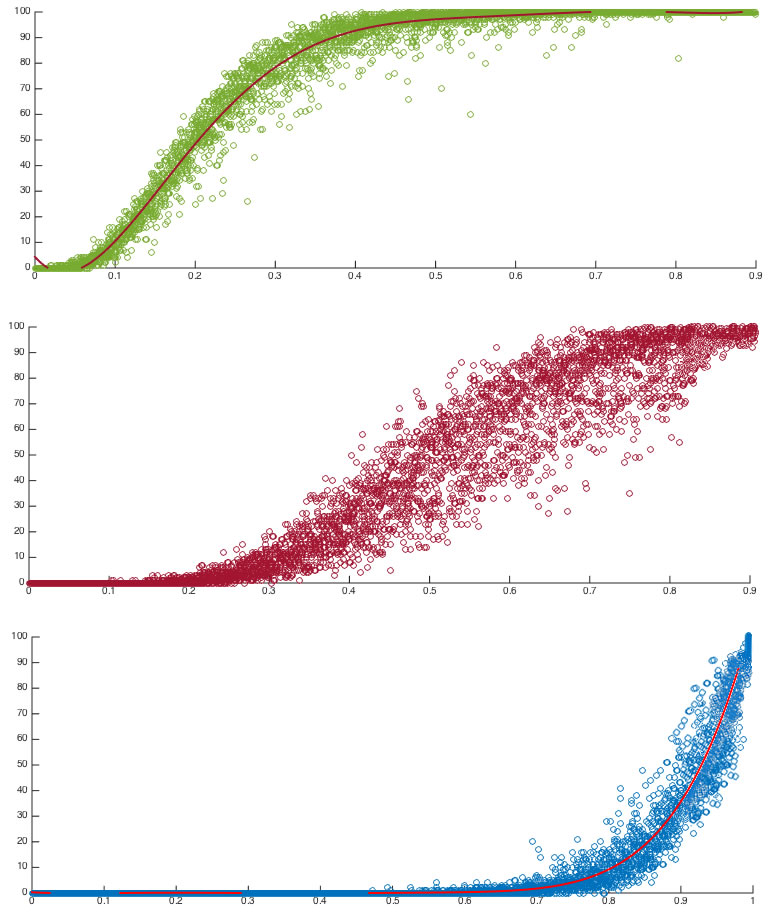
\includegraphics[scale=0.5]{Images/RandSim1.jpg}
\end{center}
\caption[Probability distribution of a random node being an elite]{Simulation on a randomly generated network giving the probability of being an elite on the $y$-axis and the proportion of affiliations connected to on the $x$-axis. In all simulations the number of affiliations is 50. The top panel has 5 aspects; the middle panel has 10 aspects; and the bottom panel has 30 aspects.}
\label{RandSim1}
\end{figure}
\end{subappendices}
